% === DEN Brand Colors ===
\usepackage{xcolor}
\definecolor{denbrown}{HTML}{6A4A3C}
\definecolor{dendark}{HTML}{2B2B2B}
\definecolor{dengray}{HTML}{F2F2F2}

% === Required Packages ===
\usepackage{tikz}
\usepackage{graphicx}
\usepackage{calc}

% Preserve aspect ratio on all \includegraphics by default. fig-height.lua sets
% a per-image height=0.65\textheight; without this, supplying both width and
% height would distort the image.
\setkeys{Gin}{keepaspectratio=true}

% === Beamer Theme Settings ===
\usetheme{default}
\usecolortheme{default}

% Remove navigation symbols
\setbeamertemplate{navigation symbols}{}

% === Font Settings ===
\usefonttheme{professionalfonts}
\setbeamerfont{title}{size=\LARGE, series=\bfseries}
\setbeamerfont{frametitle}{size=\large, series=\bfseries}
\setbeamerfont{framesubtitle}{size=\normalsize}

% === Color Settings ===
\setbeamercolor{normal text}{fg=dendark}
\setbeamercolor{frametitle}{fg=dendark}
\setbeamercolor{title}{fg=white}
\setbeamercolor{author}{fg=white}
\setbeamercolor{date}{fg=white}
\setbeamercolor{item}{fg=denbrown}
\setbeamercolor{itemize item}{fg=denbrown}
\setbeamercolor{enumerate item}{fg=denbrown}

% === Adaptive Title Sizing ===
\usepackage{ifthen}
\newlength{\titlewidth}
\newlength{\titlemaxwidth}

% === Title Page Template with Adaptive Sizing ===
\setbeamertemplate{title page}{
  \begin{tikzpicture}[remember picture, overlay]
    \node[anchor=center] at (current page.center) {
      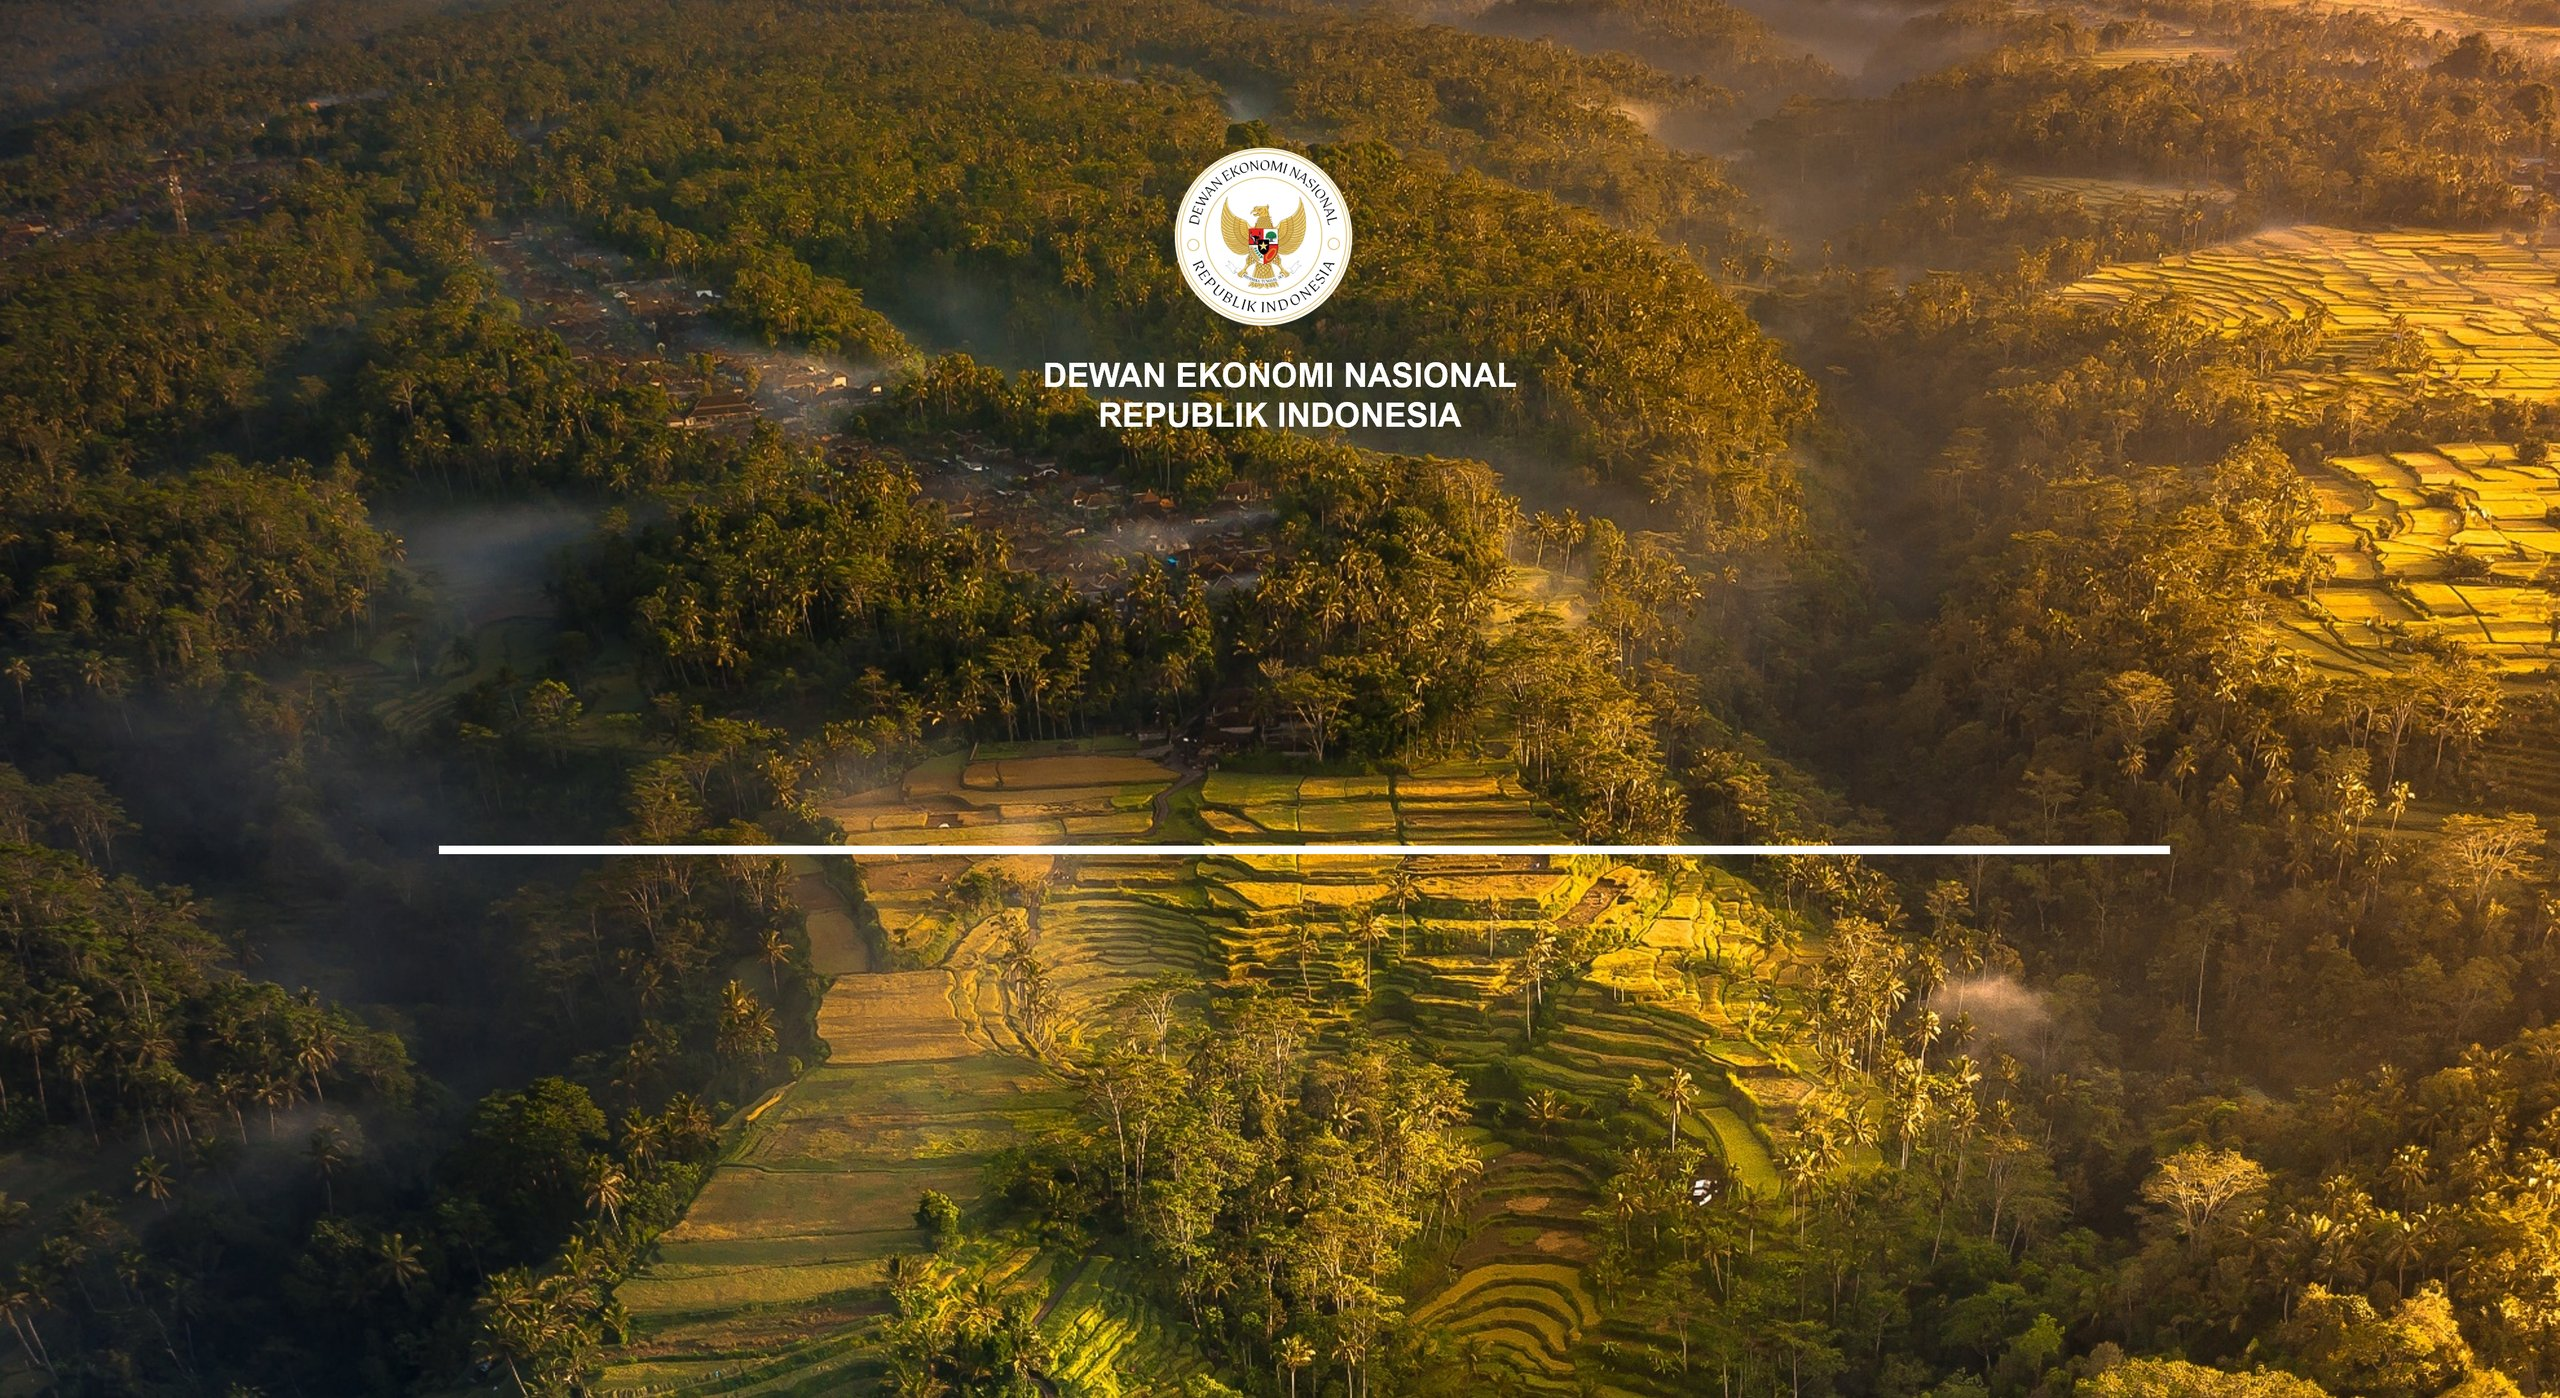
\includegraphics[width=\paperwidth, height=\paperheight, keepaspectratio=false]{title.jpg}
    };
  \end{tikzpicture}
  % Calculate title width to determine if it's long
  \setlength{\titlemaxwidth}{0.80\paperwidth}
  \settowidth{\titlewidth}{\usebeamerfont{title}\inserttitle}
  %
  \ifthenelse{\lengthtest{\titlewidth > \titlemaxwidth}}%
  {% Long title (3+ lines): 25% smaller font, higher position
    \vspace{1.8cm}
    \begin{center}
      \begin{minipage}{0.85\textwidth}
        \centering
        {\fontsize{18}{22}\selectfont\bfseries\color{white}\inserttitle\par}
        \vspace{0.3cm}
        {\usebeamerfont{author}\usebeamercolor[fg]{author}\insertauthor\par}
      \end{minipage}
    \end{center}
  }{% Short title (1 line): normal font, normal position
    \vspace{3cm}
    \begin{center}
      \begin{minipage}{0.85\textwidth}
        \centering
        {\usebeamerfont{title}\usebeamercolor[fg]{title}\inserttitle\par}
        \vspace{0.3cm}
        {\usebeamerfont{author}\usebeamercolor[fg]{author}\insertauthor\par}
      \end{minipage}
    \end{center}
  }
  \vfill
  \begin{center}
    {\usebeamerfont{date}\usebeamercolor[fg]{date}\insertdate}
  \end{center}
  \vspace{0.5cm}
}

% === Adaptive Frame Title Sizing ===
\newlength{\frametitlewidth}
\newlength{\frametitlemaxwidth}

% === Frame Title Template with Vertical Brown Line and Adaptive Sizing ===
\setbeamertemplate{frametitle}{
  \vspace{0.4cm}
  % Calculate frametitle width to determine if it's long
  \setlength{\frametitlemaxwidth}{0.75\paperwidth}
  \settowidth{\frametitlewidth}{\usebeamerfont{frametitle}\insertframetitle}
  %
  \begin{beamercolorbox}[wd=\paperwidth, leftskip=0.5cm]{frametitle}
    \tikz[baseline=-0.3ex]{
      \fill[denbrown] (0, -0.35) rectangle (0.15, 0.55);
    }
    \hspace{0.3cm}
    \ifthenelse{\lengthtest{\frametitlewidth > 1.3\frametitlemaxwidth}}%
    {% Very long title: use small font
      {\small\bfseries\insertframetitle}%
    }{%
      \ifthenelse{\lengthtest{\frametitlewidth > \frametitlemaxwidth}}%
      {% Long title: use normalsize font
        {\normalsize\bfseries\insertframetitle}%
      }{% Normal title: use standard frametitle font
        \usebeamerfont{frametitle}\insertframetitle%
      }%
    }%
  \end{beamercolorbox}
}

% === Logo in Top Right ===
\addtobeamertemplate{frametitle}{}{
  \begin{tikzpicture}[remember picture, overlay]
    \node[anchor=north east, xshift=-0.4cm, yshift=-0.2cm] at (current page.north east) {
      
\includegraphics[height=1cm]{logo.png}
    };
  \end{tikzpicture}
}

% === Footer with Page Number (Brown Box Bottom Right Corner) ===
% Hidden on title slide (frame 1)
\setbeamertemplate{footline}{%
  \ifnum\insertframenumber>1
    \begin{tikzpicture}[remember picture, overlay]
      \node[
        anchor=south east, 
        fill=denbrown, 
        text=white,
        inner sep=4pt,
        minimum width=0.6cm,
        minimum height=0.5cm,
        font=\footnotesize
      ] at (current page.south east) {
        \the\numexpr\insertframenumber-1\relax
      };
    \end{tikzpicture}
  \fi
}

% === List Item Styling ===
\setbeamertemplate{itemize item}{\textcolor{denbrown}{\textbullet}}
\setbeamertemplate{itemize subitem}{\textcolor{denbrown}{\textendash}}
\setbeamertemplate{enumerate item}{\textcolor{denbrown}{\insertenumlabel.}}

% === Block Styling ===
\setbeamercolor{block title}{bg=denbrown, fg=white}
\setbeamercolor{block body}{bg=dengray, fg=dendark}

% === Ending Slide Command ===
\providecommand{\denendslide}{
  \begin{frame}[plain]
    \begin{tikzpicture}[remember picture, overlay]
      \node[anchor=center] at (current page.center) {
        
\includegraphics[width=\paperwidth, height=\paperheight, keepaspectratio=false]{end.jpg}
      };
    \end{tikzpicture}
  \end{frame}
}

% === Support for ending-slide class via background-image attribute ===
\makeatletter
\define@key{beamerframe}{background-image}{%
  \setbeamertemplate{background}{%
    \begin{tikzpicture}[remember picture, overlay]
      \node[anchor=center] at (current page.center) {
        \includegraphics[width=\paperwidth, height=\paperheight, keepaspectratio=false]{#1}
      };
    \end{tikzpicture}
  }%
}
\makeatother

% === Section Divider Frame ===
% Full-page background image with a middle-left white title, used by
% section-divider.lua for `## Title {.section-divider background-image="..."}`
\newcommand{\denDividerFrame}[2]{%
  \begin{tikzpicture}[remember picture, overlay]
    \node[anchor=center] at (current page.center) {
      \includegraphics[width=\paperwidth, height=\paperheight, keepaspectratio=false]{#2}
    };
    \node[anchor=west, text=white, align=left, inner sep=0pt,
          text width=0.55\paperwidth]
      at ([xshift=1.2cm]current page.west)
      {\Huge\bfseries #1};
  \end{tikzpicture}%
}

% === Takeaway Box ===
% Full-text-width brown bar for the single message of a slide, used by
% takeaway.lua for `::: {.takeaway}`. The font size is fixed so the bar looks
% the same on normal, .small and .smaller slides.
\setbeamercolor{dentakeaway}{bg=denbrown, fg=white}
\newenvironment{dentakeaway}{%
  \par\vspace{0.6em}%
  \setbeamertemplate{itemize item}{\textbullet}%
  \setbeamertemplate{itemize subitem}{\textendash}%
  \begin{beamercolorbox}[wd=\textwidth, sep=7pt]{dentakeaway}%
  \small\bfseries
}{%
  \end{beamercolorbox}\par
}

% === Slot Grid and Cards ===
% Used by cols.lua for `:::: {.cols n=3}`. Each slot is typeset into one of
% the \denslotA..L boxes at a fixed width and height, then the boxes are set
% out row by row. dencard is a cream box; dencardtitle adds a coloured title
% bar; denplain is an invisible box for text or a figure.
\definecolor{dengold}{HTML}{C8860D}
\definecolor{dendarkbrown}{HTML}{3D2B1F}
\definecolor{dencream}{HTML}{F2EBDD}
\definecolor{denline}{HTML}{DDD0B8}

\usepackage{tcolorbox}
\tcbuselibrary{skins}
\tcbset{
  denslot/.style={
    nobeforeafter, valign=top, halign=flush left,
    before upper={\setlength{\parskip}{0.35em}\setlength{\leftmargini}{1.1em}},
  },
  dencard/.style={
    denslot, colback=dencream, colframe=denline, coltext=dendark,
    boxrule=0.4pt, arc=1.5pt, boxsep=0pt,
    left=5pt, right=5pt, top=4pt, bottom=4pt,
  },
  dencardtitle/.style={
    colframe=#1, colbacktitle=#1, coltitle=white,
    toptitle=1pt, bottomtitle=1pt,
  },
  denplain/.style={denslot, blanker},
}
\newsavebox{\denslotA}\newsavebox{\denslotB}\newsavebox{\denslotC}\newsavebox{\denslotD}
\newsavebox{\denslotE}\newsavebox{\denslotF}\newsavebox{\denslotG}\newsavebox{\denslotH}
\newsavebox{\denslotI}\newsavebox{\denslotJ}\newsavebox{\denslotK}\newsavebox{\denslotL}

% === Columns Stay Inside the Text Width ===
% Pandoc writes \begin{columns}[T], which lets beamer spread the columns into
% both side margins. Adding onlytextwidth keeps them aligned with the text.
\makeatletter
\let\den@columns\columns
\renewcommand{\columns}[1][]{\den@columns[#1,onlytextwidth]}
\makeatother

% === Table Styling ===
% Row padding keeps multi-line rows apart; rules are brown, heavier at the
% top and bottom. table-style.lua puts \dentablehead in every header cell.
\usepackage{booktabs}
\usepackage{colortbl}
\renewcommand{\arraystretch}{1.3}
\arrayrulecolor{denbrown}
\setlength{\heavyrulewidth}{0.9pt}
\setlength{\lightrulewidth}{0.4pt}
\newcommand{\dentablehead}{\color{denbrown}\bfseries}

% === Small Slide Classes for Heavy Content ===
% \small and \footnotesize are used via Lua filter
% These environments provide additional control if needed
\newenvironment{smallslide}{\small}{}
\newenvironment{smallerslide}{\footnotesize}{}
